\subsection{Run to failure}
\label{section:plotOverTime}
As already discussed in chapter \ref{section:TimePlotVsFingerprint}, a healthy and faulty state look visually different in the fingerprint. Looking at the healthy initial phase and comparing it to any faulty plot is enough to conclude that there is definitely some issue with the machine. To further explore how such a run to failure looks like all three tests are run on all files with a window size which spans over the entire snapshot file.
Figures~\ref{fig:runFailure1}, ~\ref{fig:runFailure2}, ~\ref{fig:runFailure3}
show the resulting fingerprints of all three independent run to failure experiments by \ref{app:appendix2}.  

\begin{figure}[H]
    \centering
    \begin{adjustwidth}{-2cm}{-2cm}  % je 2cm links und rechts in den Rand hinein
        \centering
        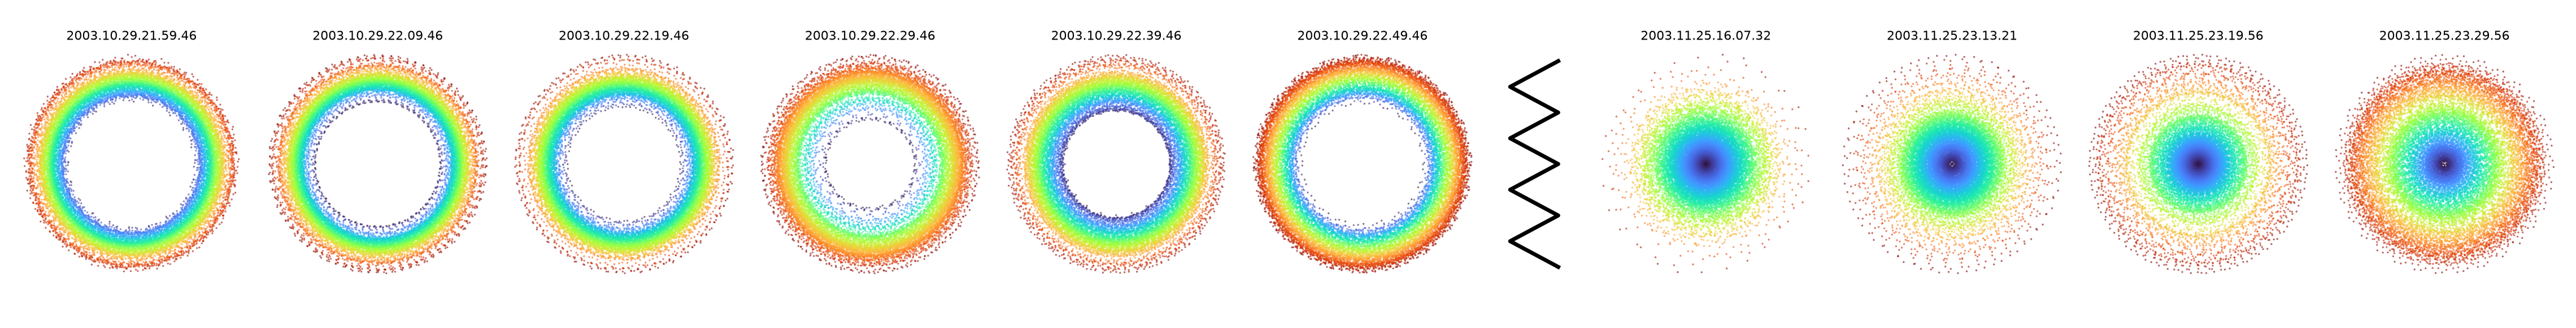
\includegraphics[width=\linewidth]{figures/runToFailure/run_to_failure_1st.png}
    \end{adjustwidth}
    \caption{Run to failure. }
    \label{fig:runFailure1}
\end{figure}

\begin{figure}[H]
    \centering
    \begin{adjustwidth}{-2cm}{-2cm}  % je 2cm links und rechts in den Rand hinein
        \centering
        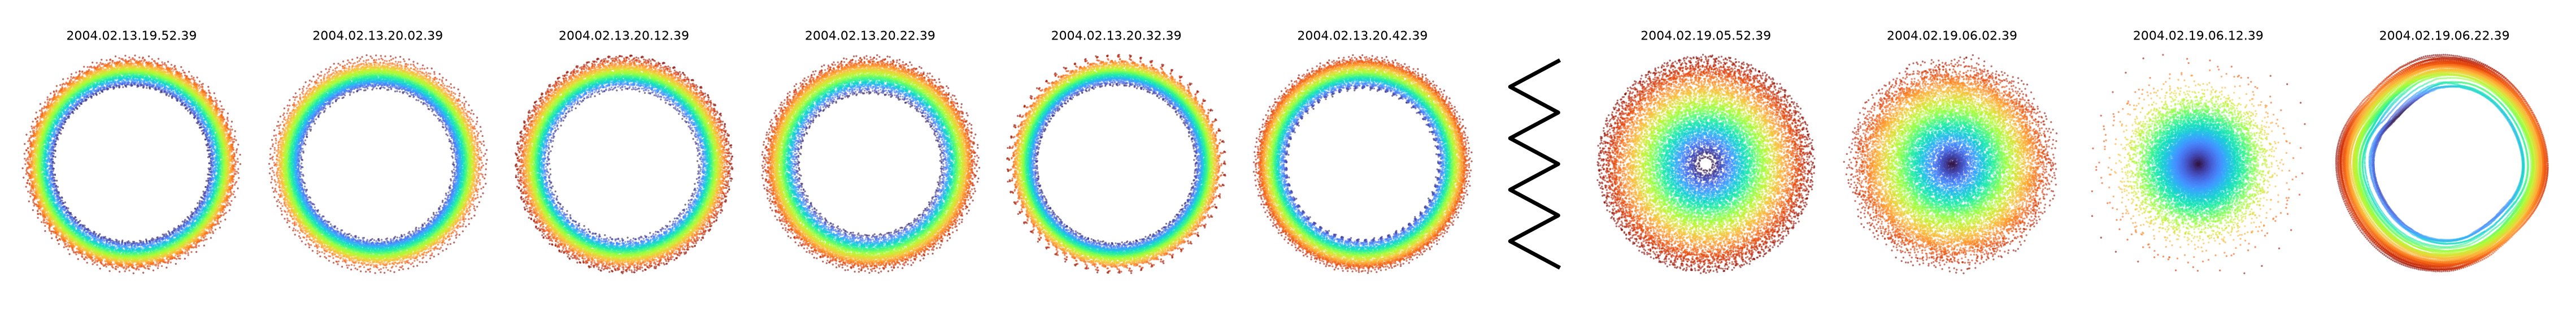
\includegraphics[width=\linewidth]{figures/runToFailure/run_to_failure_2nd.png}
    \end{adjustwidth}
    \caption{Run to failure. }
    \label{fig:runFailure2}
\end{figure}
In run one and two, the fingerprints of the healthy phase share a similar shape which is a clear and continuous ring. This rings collapse into a filled point cloud after some time iterations. The behavior in this critical section is further explained in section \ref{section:transitionToFaultyState}.
This matches the observation of \textcite{rakuschek2025visual}: noise accumulates near the center while vibrations cause the circular patterns with a larger radius
than noise. A direct mechanical defect in the bearing produces sudden impacts which overlap with the periodic vibration of the shaft. The result of this behavior is that the two dominant principal components no longer describe a single dominant oscillation but rather a mix of frequencies. Since the variance of the signal is spread over many directions of the embedding space instead of being concentrated into two main directions the projection onto the two principal components no longer form a ring but a point cloud in which most of the points lie close to the center.
With this knowledge at the beginning of the run a reference can be established that indicates faults when other fingerprints clearly distinguishes from this baseline.
\begin{figure}[H]
    \centering
    \begin{adjustwidth}{-2cm}{-2cm}  % je 2cm links und rechts in den Rand hinein
        \centering
        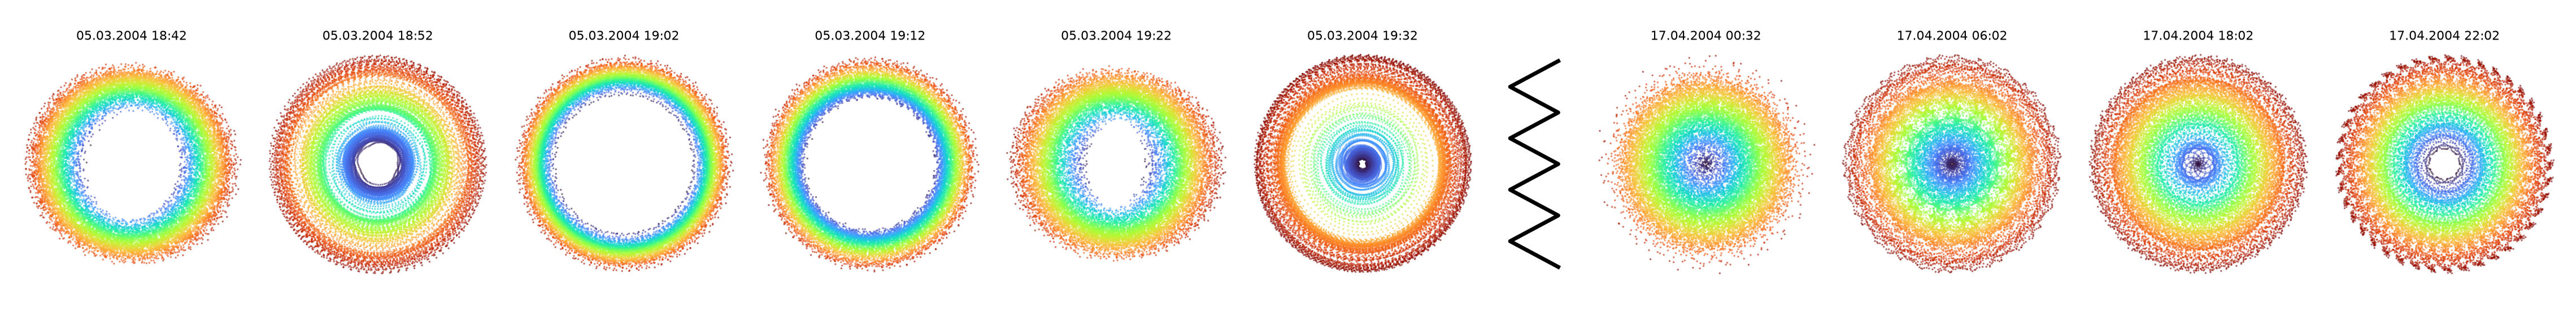
\includegraphics[width=\linewidth]{figures/runToFailure/run_to_failure_3rd.png}
    \end{adjustwidth}
    \caption{Run to failure. }
    \label{fig:runFailure3}
\end{figure}
The third dataset is not as suitable to use for the algorithm because its fingerprints show no clear initial healthy start phase at the beginning of the run as visualized in \ref{fig:runFailure3}. A closer look at the raw vibration data showed that the healthy segments of the initial signal varies within this single file which produces several rings rather than one. This can be seen in the plots of 05.03.2004 18:52 05.03.2004 19:22 and 05.03.2004 19:32. The definition on what defines a suitable dataset is left open for further discussion and will not be covered in this thesis.

